\chapter{Quellcodes zur Arbeit}
\label{app:sourcecode}
In der Arbeit werden verschiedene Quellcodes referenziert. Es folgt eine Auflisting der Quellcodes, die in der Arbeit verwendet wurden, und wo sie zu finden sind.
\begin{itemize}
    \item \textbf{Quellcode des Dashboards}: Der Quellcode des Dashboards ist in einem Git-Repository auf GitLab verfügbar. Dieselbe Gitlab-Instanz enthält auch die Projekte und Quellcodes für andere Komponenten des Forschungsprojekts. Zum aktuellen Zeitpunkt ist der Zugriff auf das Repository nur für autorisierte Personen möglich. Das Forschungsprojekt verfolgt das Ziel, alle Quellcodes nach Abschluss des Projekts zu veröffentlichen, voraussichtlich im ersten Halbjahr des Jahres 2025. Der genaue Link zum Repository wird zu gegebener Zeit unter \url{https://www.5g-foran.com/} veröffentlicht.
    \item \textbf{Quellcode von \citeauthor{klementSecuring6GTransition2024}}: Der Quellcode der Implementation von \citeauthor{klementSecuring6GTransition2024} ist in einem Git-Repository auf GitHub verfügbar. Im Fließtext dieser Arbeit wird dieser Quelltext als \textit{originaler Quellcode} bezeichnet. Der Quellcode ist unter folgendem Link verfügbar: \url{https://github.com/fklement/acema_oran}
    \item \textbf{Fork des Quellcode von \citeauthor{klementSecuring6GTransition2024}}: Der Quellcode des Forks von \citeauthor{klementSecuring6GTransition2024} ist in einem Git-Repository auf GitHub verfügbar. Der Fork enthält die eigens vorgenommenen Änderungen und wird im Fließtext dieser Arbeit als \textit{verbesserter Quellcode} bezeichnet. Der Quellcode ist unter folgendem Link verfügbar: \url{https://github.com/dumpeldown/acema_oran}
\end{itemize}


\chapter{Ausschnitt aus dem ACEMA-Output}
\label{app:acema-output}
\newgeometry{left=1cm, right=1cm}
\verbatiminput{data/acema-output.json}
\restoregeometry
\chapter{Ausschnitt aus dem angepassten ACEMA-Output}
\label{app:acema-output-small}
\newgeometry{left=1cm, right=1cm}
\verbatiminput{data/acema-output-small.json}
\restoregeometry

\chapter{Mapping Datensatz}
\newgeometry{left=1cm, right=1cm}
\label{app:mapping-dataset}
\begin{longtable}{|l|l|l|l|l|}
    \caption{Mapping von Threat-ID zu MITRE-Technik und MITRE-Taktik}\\
    \hline
    Threat-ID & TK4M Technique Name & MITRE-Technique & MITRE-Technique \\ \hline
T-IMG-01 & Application Vulnerability & T1190 & initial-access \\ \hline
T-VM-C-01 & bash or cmd inside container & T1059 & execution \\ \hline
T-VM-C-01 & bash or cmd inside container & T1204 & execution \\ \hline
T-ADMIN-02 & bash or cmd inside container & T1059 & execution \\ \hline
T-ADMIN-02 & bash or cmd inside container & T1204 & execution \\ \hline
T-HW-01 & bash or cmd inside container & T1059 & execution \\ \hline
T-HW-01 & bash or cmd inside container & T1204 & execution \\ \hline
T-IMG-01 & bash or cmd inside container & T1059 & execution \\ \hline
T-IMG-01 & bash or cmd inside container & T1204 & execution \\ \hline
T-VM-C-01 & Kubernetes CronJob & T1053.007 & persistence \\ \hline
T-VM-C-01 & Clear container logs & T1070 & defense-evasion \\ \hline
T-IMG-01 & Compromised Image In Registry & T1195.002 & initial-access \\ \hline
T-IMG-01 & Compromised Image In Registry & T1525 & initial-access \\ \hline
T-GEN-02 & Access Managed Identity credentials & T1552 & credential-access \\ \hline
T-O2-01 & Network mapping & T1046 & discovery \\ \hline
T-VM-C-02 & Cluster internal networking & T1210 & lateral-movement \\ \hline
T-IMG-01 & images from a private registry & T1530 & collection \\ \hline
T-IMG-04 & images from a private registry & T1530 & collection \\ \hline
T-ADMIN-02 & Exec into container & T1609 & execution \\ \hline
T-O2-01 & Exec into container & T1609 & execution \\ \hline
T-VM-C-03 & Exec into container & T1609 & execution \\ \hline
T-VM-C-04 & Exec into container & T1609 & execution \\ \hline
T-VM-C-01 & Backdoor container & T1543 & persistence \\ \hline
T-VM-C-01 & Backdoor container & T1542 & persistence \\ \hline
T-VL-02 & Backdoor container & T1543 & persistence \\ \hline
T-VL-02 & Backdoor container & T1542 & persistence \\ \hline
T-GEN-02 & Mount service principal & T1552 & credential-access \\ \hline
T-O2-01 & Access Kubelet API & T1613 & discovery \\ \hline
T-IMG-03 & List K8S secrets & T1552 & credential-access \\ \hline
T-VM-C-04 & Resource hijacking & T1496 & impact \\ \hline
T-VL-01 & Resource hijacking & T1496 & impact \\ \hline
T-O2-01 & Delete K8S events & T1070 & defense-evasion \\ \hline
T-VL-01 & Pod or container name similarily & T1036 & defense-evasion \\ \hline
T-VL-01 & Pod or container name similarily & T1036.005 & defense-evasion \\ \hline
T-IMG-01 & Pod or container name similarily & T1036 & defense-evasion \\ \hline
T-IMG-01 & Pod or container name similarily & T1036.005 & defense-evasion \\ \hline
T-ADMIN-01 & Denial of service & T1498 & impact \\ \hline
T-ADMIN-01 & Denial of service & T1499 & impact \\ \hline
T-VM-C-04 & Denial of service & T1498 & impact \\ \hline
T-VM-C-04 & Denial of service & T1499 & impact \\ \hline
T-VM-C-05 & Denial of service & T1498 & impact \\ \hline
T-VM-C-05 & Denial of service & T1499 & impact \\ \hline
T-GEN-02 & container service account & T1528 & credential-access \\ \hline
T-GEN-02 & container service account & T1528 & lateral-movement \\ \hline
T-GEN-02 & container service account & T1528 & persistence \\ \hline
T-ADMIN-02 & Application credentials in configuration files & T1552 & credential-access \\ \hline
T-VM-C-03 & Application credentials in configuration files & T1552 & credential-access \\ \hline
T-ADMIN-02 & Application credentials in configuration files & T1552 & lateral-movement \\ \hline
T-VM-C-03 & Application credentials in configuration files & T1552 & lateral-movement \\ \hline
T-VM-C-03 & Instance Metadata API & T1552 & discovery \\ \hline
T-IMG-03 & Instance Metadata API & T1552 & discovery \\ \hline
T-VM-C-01 & Data destruction & T1485 & impact \\ \hline
T-GEN-01 & Application exploit (RCE) & T1190 & execution \\ \hline
T-VM-C-01 & Privileged container & T1610 & privilege-escalation \\ \hline
T-VM-C-02 & Writable hostPath mount & T1611 & persistence \\ \hline
T-VM-C-02 & Writable hostPath mount & T1611 & privilege-escalation \\ \hline
T-VM-C-02 & Writable hostPath mount & T1611 & lateral-movement \\ \hline
T-O2-01 & Access the K8S API server & T1613 & discovery \\ \hline
T-GEN-02 & Exposed sensitive interfaces & T1133 & initial-access \\ \hline
T-GEN-02 & Exposed sensitive interfaces & T1078 & initial-access \\ \hline
T-GEN-02 & Exposed sensitive interfaces & T1133 & discovery \\ \hline
T-GEN-02 & Exposed sensitive interfaces & T1078 & discovery \\ \hline
T-IMG-01 & New Container & T1610 & execution \\ \hline
T-IMG-01 & New Container & T1612 & execution \\ \hline
T-IMG-04 & New Container & T1610 & execution \\ \hline
T-IMG-04 & New Container & T1612 & execution \\ \hline
\end{longtable}
\restoregeometry


\chapter{Datenstruktur}
\label{app:db-schema}

\begin{figure}[!htb]
    \centering
    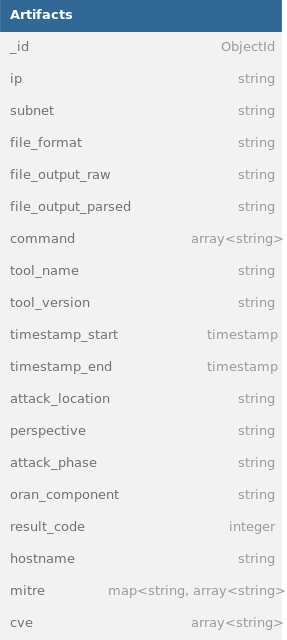
\includegraphics[width=0.5\textwidth]{db-schema}
    \caption{Struktur eines Artefakts in der Datenbank und in Go.}
\end{figure}

\chapter{Angepasste Matrix im Dashboard}
\label{app:matrix}
\begin{figure}[!htb]
    \centering
    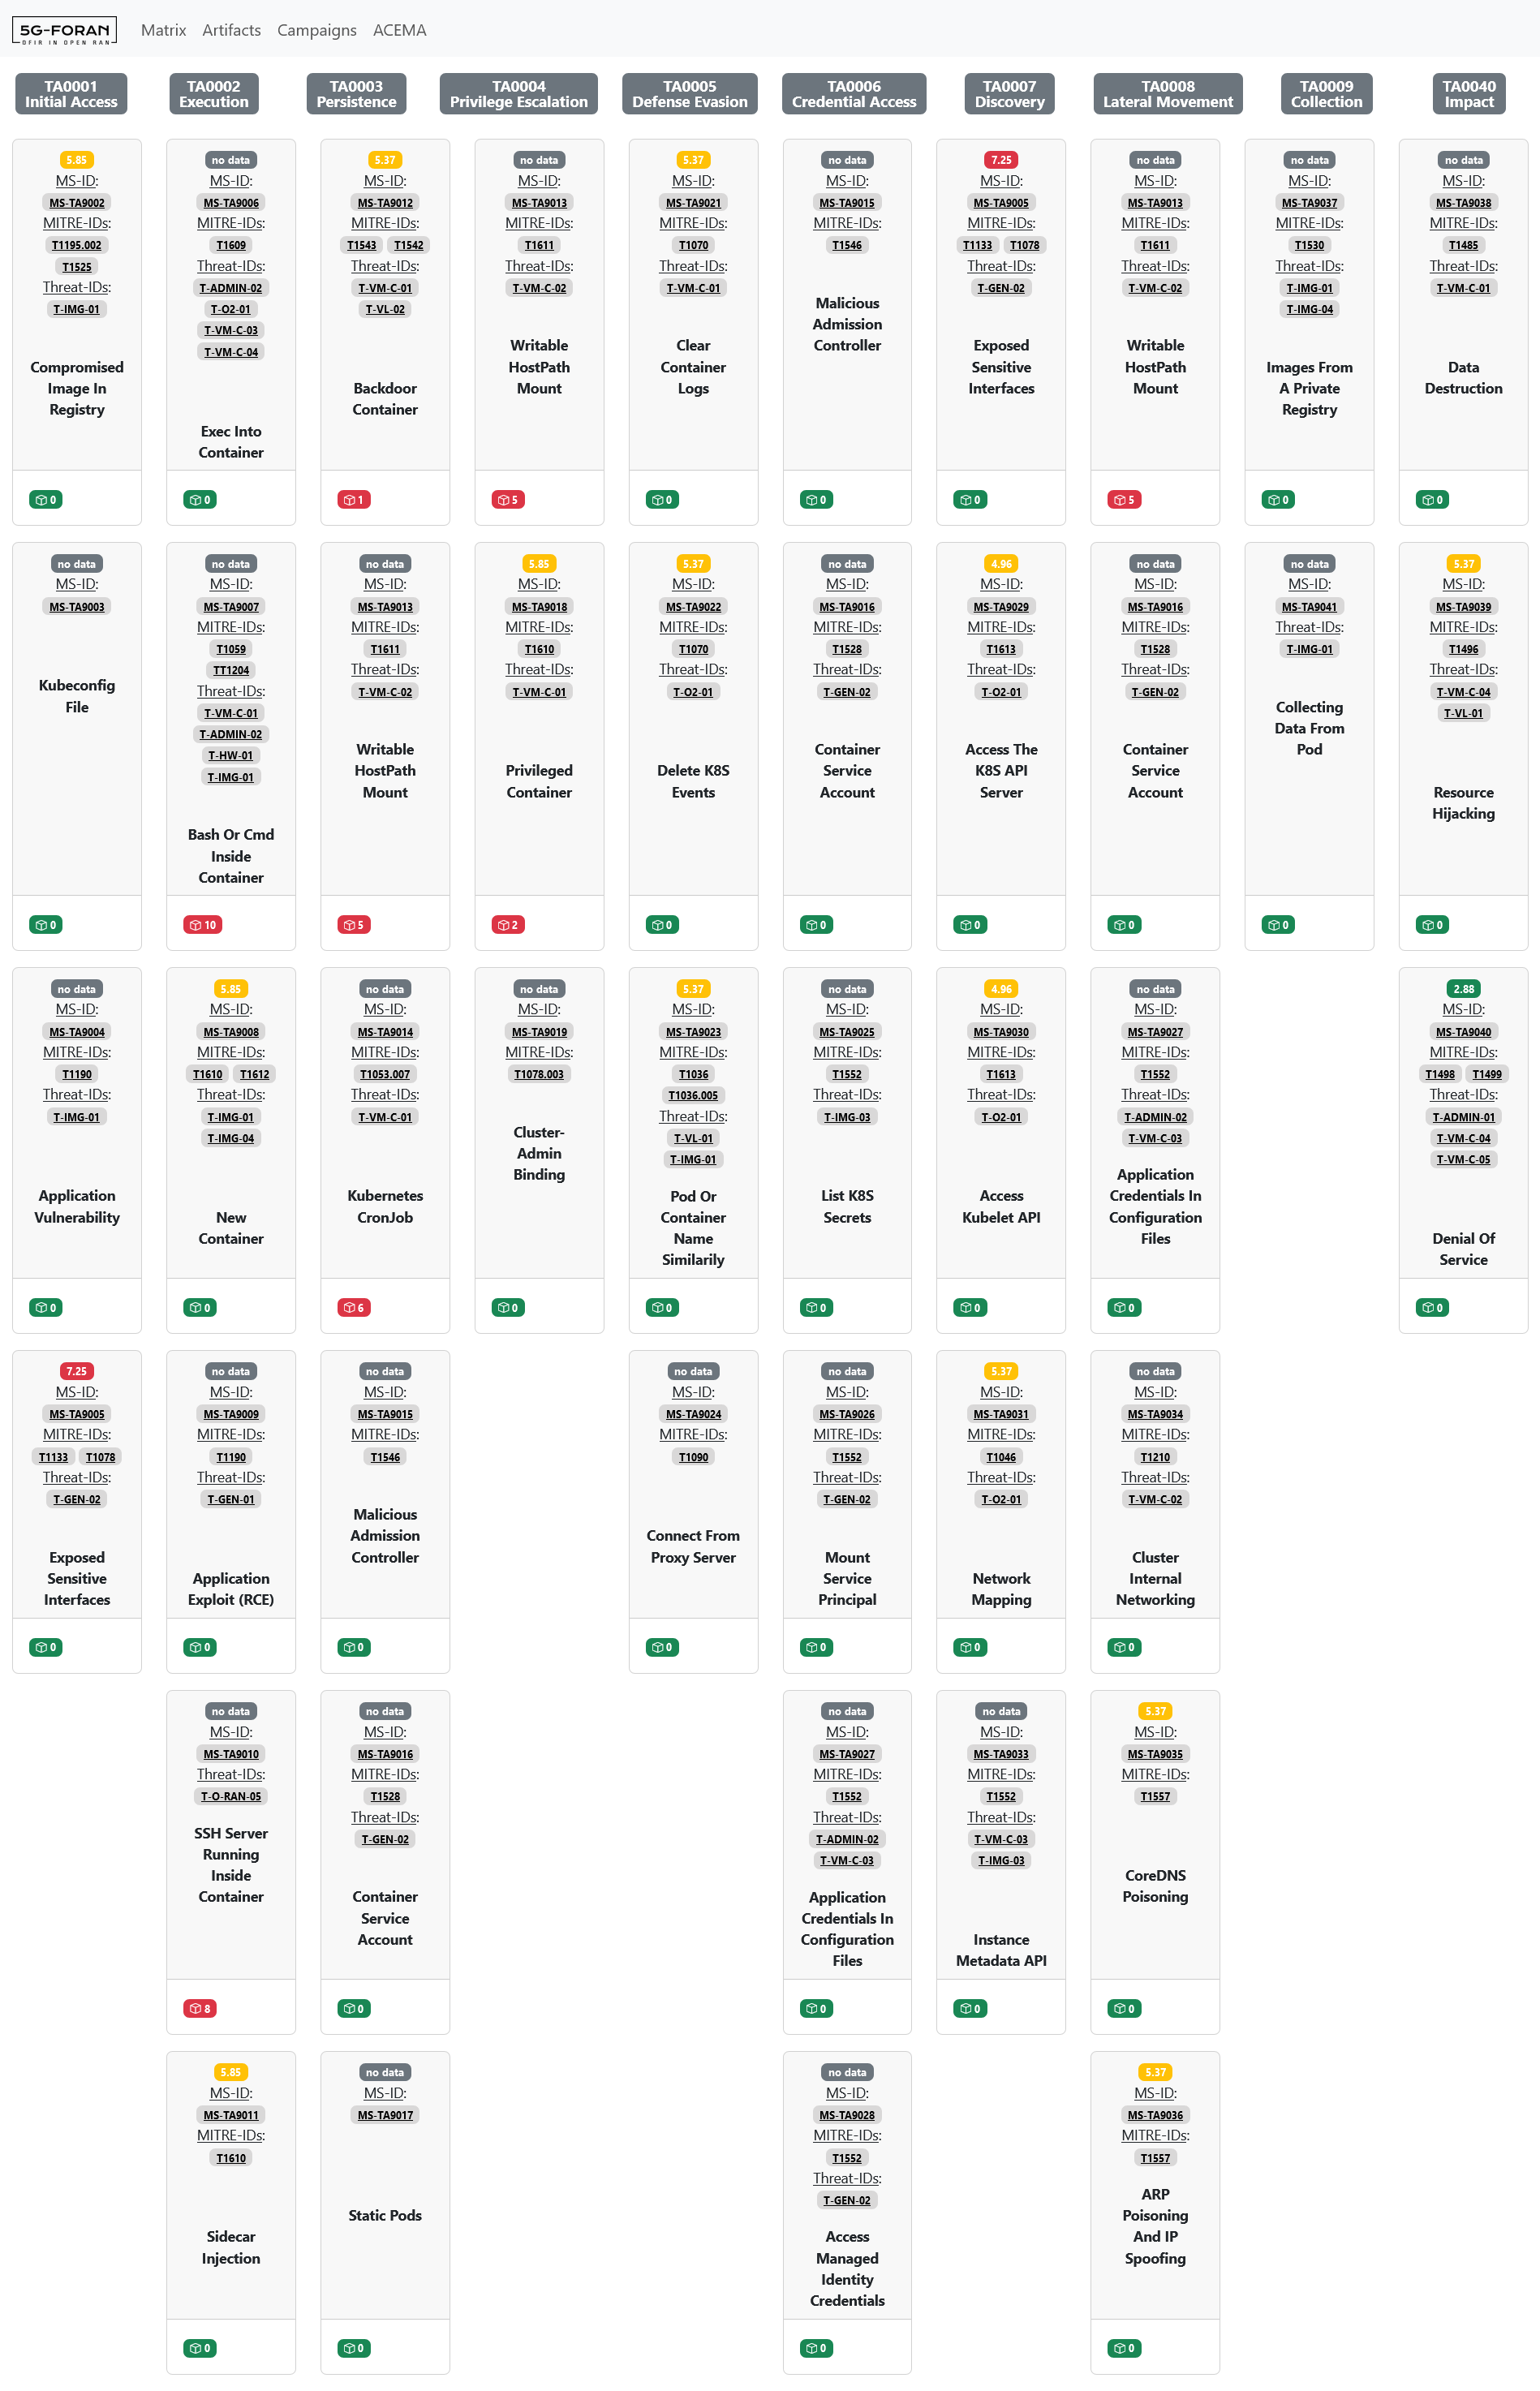
\includegraphics[width=1\textwidth]{matrix}
    \caption{Darstellung aller Techniken in der Matrix.}
\end{figure}

\chapter{Diagramme aus ACEMA}
\label{app:acema-diagrams}
Die Werte der Metriken in einem \gls{cvss}Version 2 Vektor werden typischerweise nicht numerisch, sondern textuell ausgedrückt. Um mit den Werten zu rechnen, wird die textuelle Darstellung über Formeln in einen numerischen Wert umgewandelt, die in der \gls{cvss}Version 2 Spezifikation hinterlegt sind \autocite{CVSSV2Complete}. Diese Werte werden in der \gls{acema} Implementation genutzt, um die Werte in einem Spektrum zwischen 0 und 1 darzustellen, um diese in einem Netzdiagram darzustellen (vgl. Abbildung \ref{app:fig-acema-radar}).
\[
\begin{aligned}
\text{AccessVector} & = 
\begin{cases} 
    \text{requires local access} & : 0{,}395 \\
    \text{adjacent network accessible} & : 0{,}646 \\
    \text{network accessible} & : 1{,}0
\end{cases} \\[10pt]
\text{AccessComplexity} & = 
\begin{cases} 
    \text{high} & : 0{,}35 \\
    \text{medium} & : 0{,}61 \\
    \text{low} & : 0{,}71
\end{cases} \\[10pt]
\text{Authentication} & = 
\begin{cases} 
    \text{requires multiple instances of authentication} & : 0{,}45 \\
    \text{requires single instance of authentication} & : 0{,}56 \\
    \text{requires no authentication} & : 0{,}704
\end{cases} \\[10pt]
\text{ConfImpact} & = 
\begin{cases} 
    \text{none} & : 0{,}0 \\
    \text{partial} & : 0{,}275 \\
    \text{complete} & : 0{,}660
\end{cases} \\[10pt]
\text{IntegImpact} & = 
\begin{cases} 
    \text{none} & : 0{,}0 \\
    \text{partial} & : 0{,}275 \\
    \text{complete} & : 0{,}660
\end{cases} \\[10pt]
\text{AvailImpact} & = 
\begin{cases} 
    \text{none} & : 0{,}0 \\
    \text{partial} & : 0{,}275 \\
    \text{complete} & : 0{,}660
\end{cases}
\end{aligned}
\]


\begin{figure}[!htb]
    \begin{adjustbox}{addcode={
        \begin{minipage}{\width}}{
            \caption{Durchschnittlicher CVSS Vektor aller CVEs pro Schweregrad}
        \end{minipage}}}
        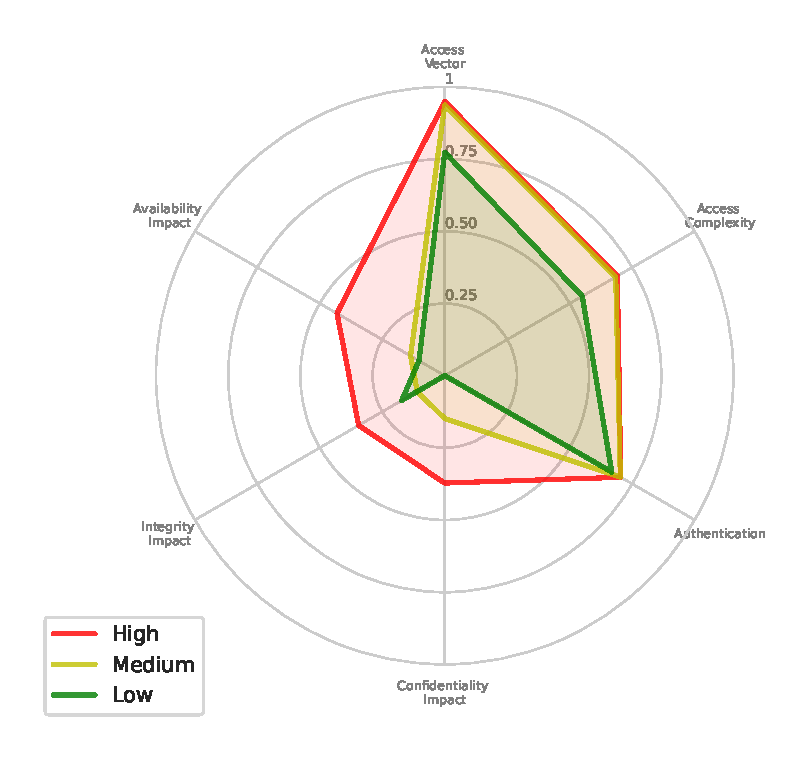
\includegraphics[scale=1]{data/radar_plot_vector_per_severity.pdf}
    \end{adjustbox}
    \label{app:fig-acema-radar}
\end{figure}

\begin{figure}[!htb]
    \begin{adjustbox}{addcode={
        \begin{minipage}{\width}}{
            \caption{Durchschnitt aller CVSS Werte der CVEs pro MITRE-Technik und Schweregrad}
        \end{minipage}},rotate=-90,center}
        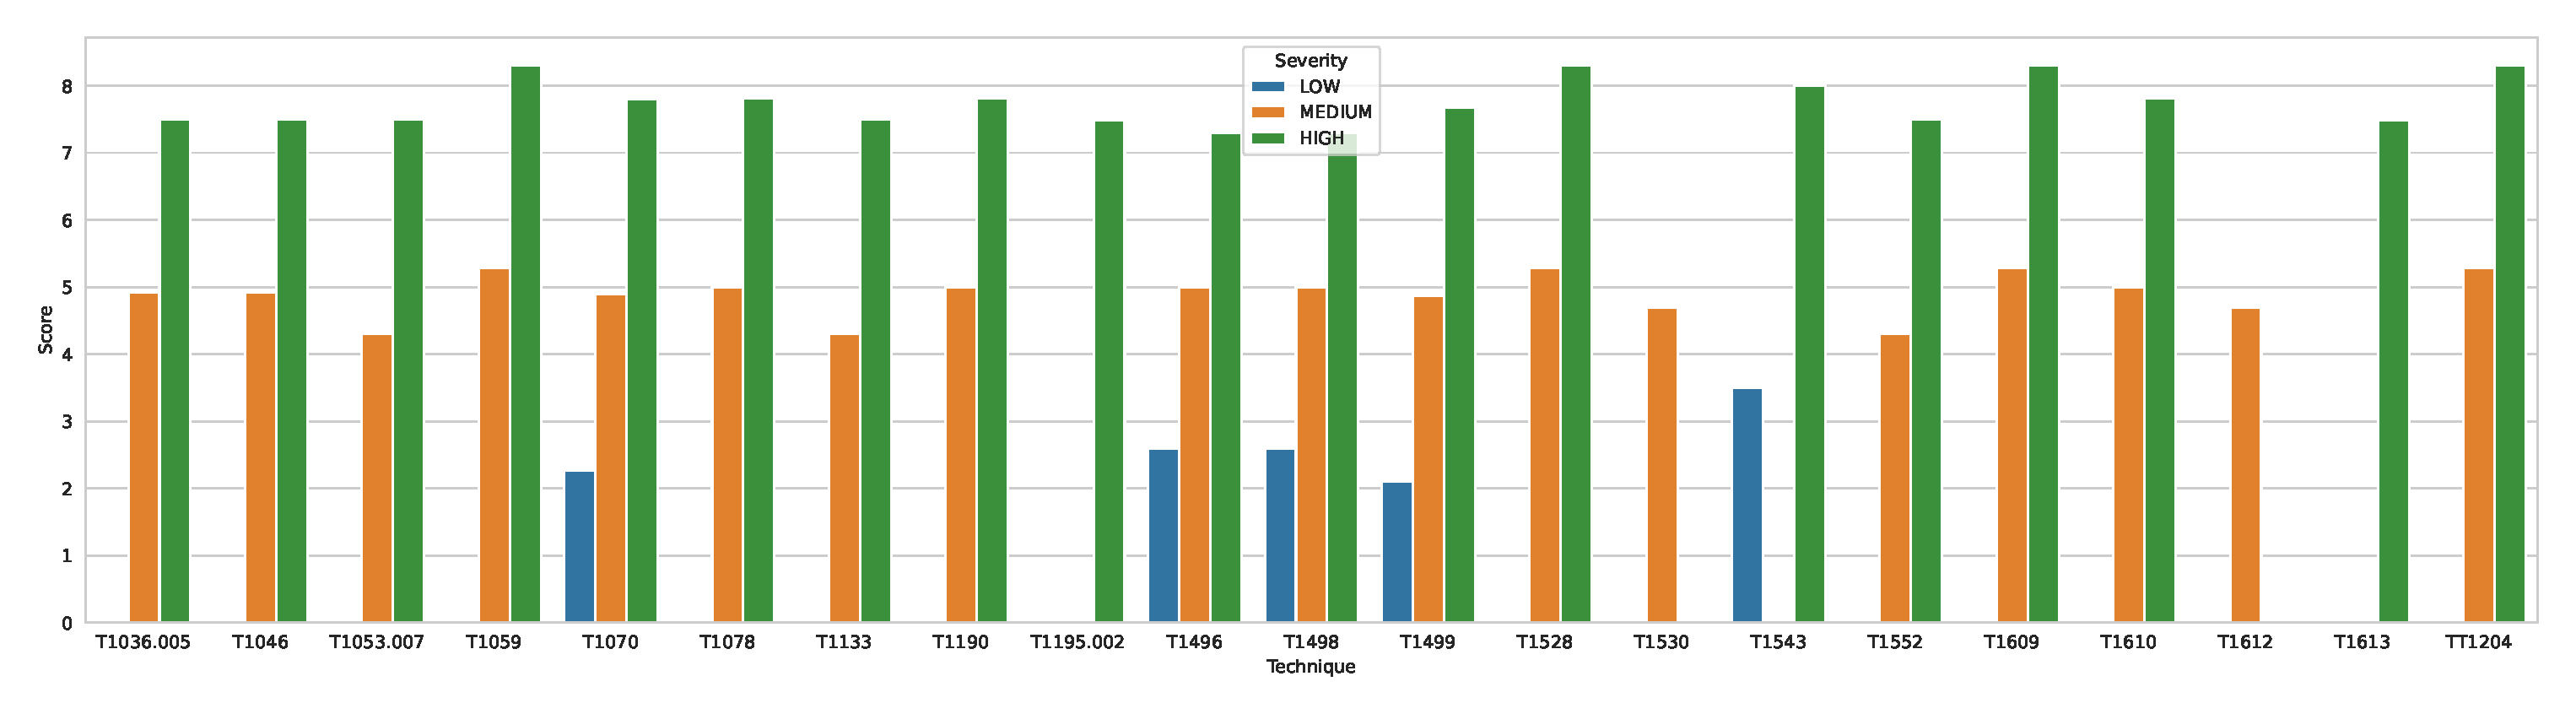
\includegraphics[scale=0.5]{data/mean_cvss_scores_per_technique_and_sev.pdf}
    \end{adjustbox}
    \label{app:fig-acema-mean-teq}
\end{figure}

\begin{figure}[!htb]
    \begin{adjustbox}{addcode={
        \begin{minipage}{\width}}{
            \caption{Summierung aller CVSS Werte der CVEs pro O-RAN Threat-ID und Schweregrad}
        \end{minipage}},rotate=-90,center}
        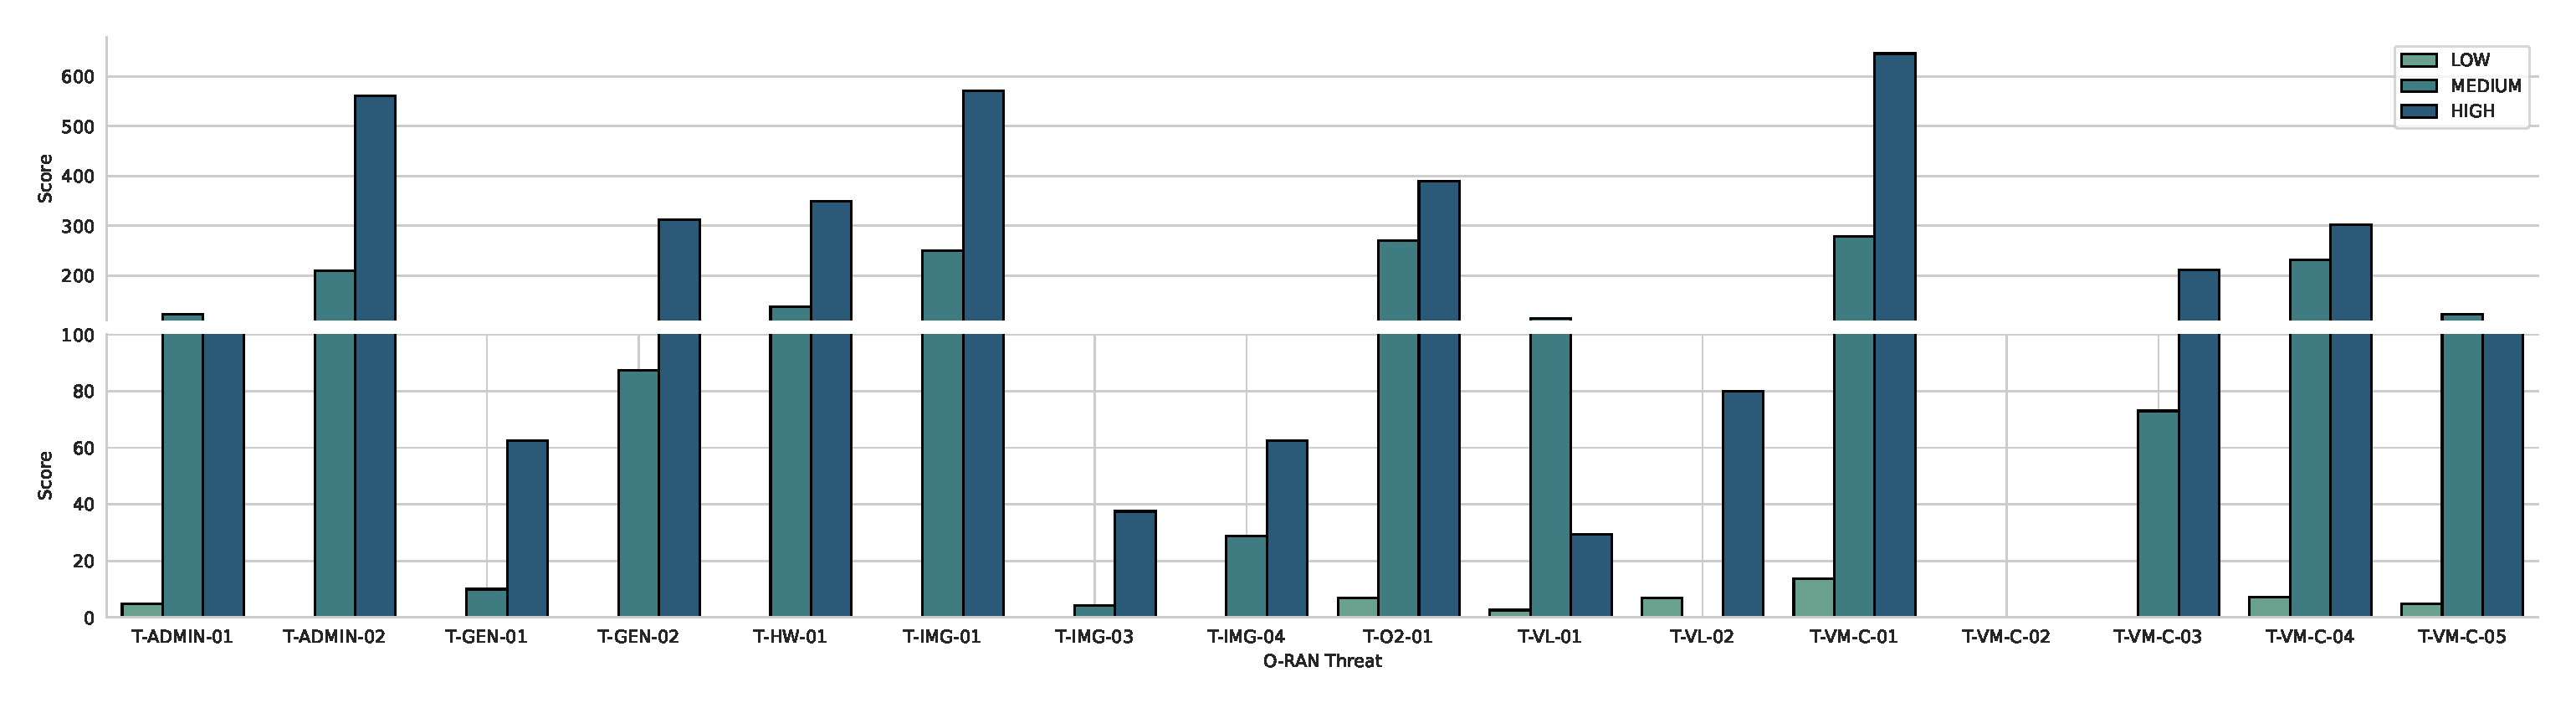
\includegraphics[scale=0.5]{data/sum_of_cvss_scores_per_threat_and_sev.pdf}
    \end{adjustbox}
    \label{app:fig-acema-sum-threat}
\end{figure}


